\documentclass[border=5pt]{standalone}
\usepackage[european,americaninductors]{circuitikz}
\usepackage{tikz}
\usetikzlibrary{patterns}
\begin{document}
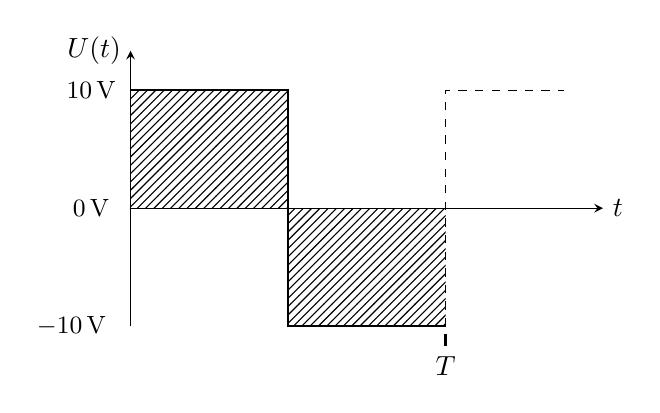
\begin{tikzpicture}[>=stealth]

% Achsen
\draw[->] (0,-1.5) -- (0,2) node[left] {$U(t)$};
\draw[->] (0,0) -- (6,0) node[right] {$t$};

% Signallinien
\draw[thick] 
    (0,1.5) -- (2,1.5) -- (2,-1.5) -- (4,-1.5);
\draw[dashed] 
    (4, -1.5) -- (4,1.5) -- (5.5,1.5);

% Schraffuren
\fill[pattern=north east lines] (0,0) rectangle (2,1.5);
\fill[pattern=north east lines] (2,-1.5) rectangle (4,0);

% Beschriftungen
\node at (-0.5,1.5) {\small $10\,\mathrm{V}$};
\node at (-0.5,0) {\small $0\,\mathrm{V}$};
\node at (-0.75,-1.5) {\small $-10\,\mathrm{V}$};

% T Markierung
\draw[thick] (4,-1.6) -- (4,-1.75);
\node at (4,-2) {$T$};

\end{tikzpicture}
\end{document}
